%-----------------------------------LICENSE------------------------------------%
%   This file is part of tikz_figures.                                         %
%                                                                              %
%   tikz_figures is free software: you can redistribute it and/or              %
%   modify it it under the terms of the GNU General Public License as          %
%   published by the Free Software Foundation, either version 3 of the         %
%   License, or (at your option) any later version.                            %
%                                                                              %
%   tikz_figures is distributed in the hope that it will be useful,            %
%   but WITHOUT ANY WARRANTY; without even the implied warranty of             %
%   MERCHANTABILITY or FITNESS FOR A PARTICULAR PURPOSE.  See the              %
%   GNU General Public License for more details.                               %
%                                                                              %
%   You should have received a copy of the GNU General Public License along    %
%   with tikz_figures.  If not, see <https://www.gnu.org/licenses/>.           %
%------------------------------------------------------------------------------%

% Use the standalone class for displaying the tikz image on a small PDF.
\documentclass[crop, tikz]{standalone}

% Import the tikz package to use for the drawing.
\usepackage{tikz}

% Begin the document.
\begin{document}

    % Draw the figure.
    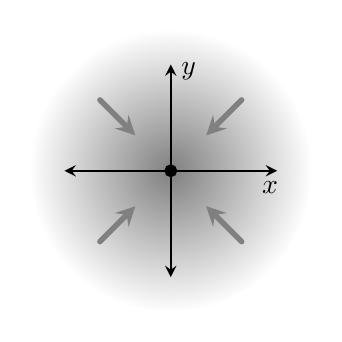
\begin{tikzpicture}[%
        scale = 0.9,
        line width = 1pt,
        line cap = round,
        > = stealth,
        every edge/.style = {%
            draw = black,
            very thick
        },
        grayarrow/.style = {%
            > = stealth,
            fill = gray,
            draw = gray,
            line width = 0.7mm,
            ->
        }
    ]
        \filldraw[%
            even odd rule,
            inner color = gray,
            outer color = white,
            draw = white
        ] (0.0, 0.0) circle (2);
        \draw[thick, <->] (-1.5, 0.0) to (1.5, 0.0);
        \draw[thick, <->] (0.0, -1.5) to (0.0, 1.5);
        \draw[grayarrow] (1.0, 1.0) to (0.5, 0.5);
        \draw[grayarrow] (-1.0, -1.0) to (-0.5, -0.5);
        \draw[grayarrow] (1.0, -1.0) to (0.5, -0.5);
        \draw[grayarrow] (-1.0, 1.0) to (-0.5, 0.5);
        \draw[fill = black] (0.0, 0.0) circle (2pt);
        \node at (1.4, 0.0) [below] {$x$};
        \node at (0.0, 1.4) [right] {$y$};
    \end{tikzpicture}
\end{document}
